\documentclass[12pt]{article}
\usepackage{inputenc}
\usepackage{graphicx}
\usepackage{tabularx}
\usepackage{hyperref}

%%%%%%%%%%%%%%%%
% Impostazioni %
%%%%%%%%%%%%%%%%

\date{}

\hypersetup{
    colorlinks=true,
    linkcolor=blue,
    filecolor=magenta,
    urlcolor=cyan,
    pdftitle={Database Banca, Michael Guidelli},
    pdfpagemode=FullScreen,
}


\begin{document}

%%%%%%%%%%
% Titolo %
%%%%%%%%%%

\maketitle
\null \null \null \null \null \null
{\centering
    \huge\bfseries Database Car Sharing \\
    \Large\normalfont Michael Guidelli  \\
}

\clearpage

%%%%%%%%%%%%%%%%%%%%%
% Traccia esercizio %
%%%%%%%%%%%%%%%%%%%%%

\section*{Traccia esercizio}

\noindent
Un’associazione di car-sharing mantiene un database del parco auto e dei soci al fine di registrare i
noleggi e verificare le disponibilità delle vetture.
Ciascun socio può accedere all’intero parco macchine disponibile e naturalmente ciascuna auto può
essere noleggiata da più soci (in tempi diversi).
Si crei il modello ER, la lista degli attributi con tipo di dato, il modello logico e il DBSchema
(Create table).

\clearpage

%%%%%%%%%%%%%%%%%%%%%%%%%%%%%%%%
% Impostazioni indice e figure %
%%%%%%%%%%%%%%%%%%%%%%%%%%%%%%%%%

\renewcommand{\contentsname}{Indice \label{indice}}
\tableofcontents

\renewcommand{\listfigurename}{Lista delle figure}
\listoffigures

\renewcommand{\listtablename}{Liste Attributi}
\listoftables

\clearpage

%%%%%%%%%%%
% Ipotesi %
%%%%%%%%%%%

\section{Ipotesi}
\begin{enumerate}
    \item Ipotizzo che ogni socio possa noleggiare tutte le auto del parco auto disponibili e naturalmente ciascuna auto possa essere noleggiata da più soci in tempi diversi.
\end{enumerate}

\clearpage

%%%%%%%%%%%%%%
% Modello ER %
%%%%%%%%%%%%%%

\section{Modello ER}
\begin{figure}[h!]
    \centering
    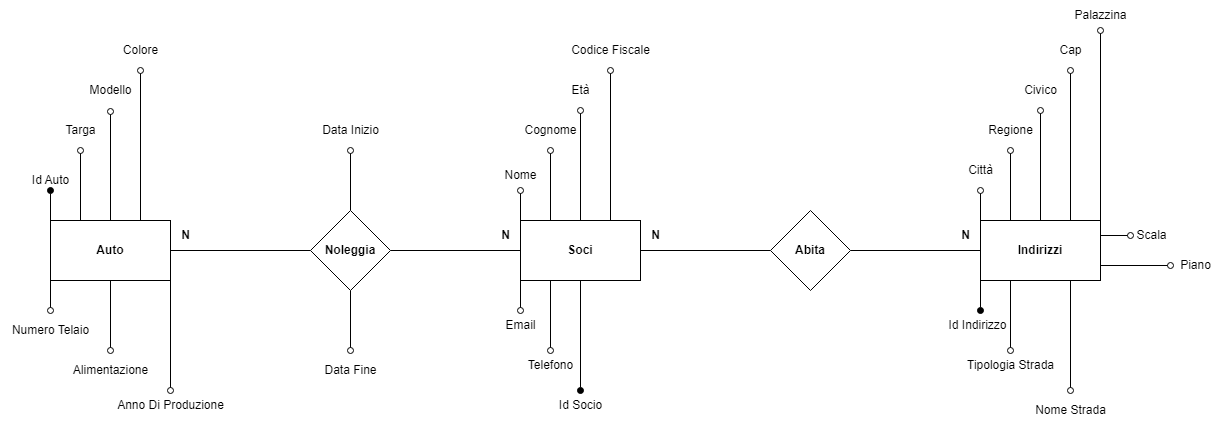
\includegraphics[width=16cm]{modello_er_car_sharing.png}
    \label{fig:modello Er}
    \caption{Rappresentazione modello ER}
\end{figure}

%%%%%%%%%%%%%%%
% Cardinalità %
%%%%%%%%%%%%%%%

\subsection{Cardinalità}

\noindent
Cardinalità delle associazioni:

\begin{itemize}
    \item \textbf{Noleggia}: La cardinalità è \textbf{N} a \textbf{N} dato che ciascun singolo socio può noleggiare \textbf{N} auto e ciascuna singola auto può essere noleggiata da \textbf{N} soci (in tempi diversi).

    \item \textbf{Abita}: La cardinalità è \textbf{N} a \textbf{N} dato che ciascun singolo socio può avere una abitazione in più indirizzi e ciascun singolo indirizzo  può essere abitato da più soci. 
\end{itemize}

\clearpage

%%%%%%%%%%%%%%%%%%%%%%%%%
% Liste degli attributi %
%%%%%%%%%%%%%%%%%%%%%%%%%

\begin{center}
    \section{Liste degli attributi}
\end{center}

% Entità Auto %
\subsection{Entità Auto}
\begin{table}[h!]
    \centering
    \begin{tabular}{|c|c|c|c|}
        \hline
        Nome attributo & Significato & Tipo di dato & Vincolo \\
        \hline
        Id Auto & Attributo identificativo & Int & \\
        \hline
        Targa & Targa Auto & Varchar & 7 caratteri \\
        \hline
        Modello & Modello Auto & Varchar & Max 255 caratteri \\ 
        \hline
        Colore & Colore Auto & Varchar &  Max 255 caratteri \\ 
        \hline
        Numero Telaio & Telaio Auto & Varchar & 17 caratteri \\
        \hline
        Alimentazione & Alimentazione Auto & Varchar & Max 255 caratteri \\
        \hline
        Anno Di Produzione & Anno di produzione auto & Date & \\
        \hline
    \end{tabular}
    \caption{Entità Auto}
    \label{tab:Entità Auto}
\end{table}

\subsection{Attributi Associazione Noleggia}
\begin{table}[h!]
    \centering
    \begin{tabular}{|c|c|c|c|}
        \hline
        Nome attributo & Significato & Tipo di dato & Vincolo \\
        \hline
        Data Inizio & Inizio noleggio & Date & \\
        \hline
        Data Fine & Fine noleggio & Date & \\
        \hline
    \end{tabular}
    \caption{Attributi associazione Noleggia}
    \label{tab:Attributi associazione Noleggia}
\end{table}

\clearpage

% Entità Soci %

\subsection{Soci}
\begin{table}[h!]
    \centering
    \begin{tabular}{|c|c|c|c|}
        \hline
        Nome attributo & Significato & Tipo di dato & Vincolo \\
        \hline
        Id Socio & Attributo identificativo & Int & \\
        \hline
        Nome & Nome socio & Varchar & Max 255 caratteri  \\
        \hline
        Cognome & Cognome socio & Varchar & Max 255 caratteri  \\
        \hline
        Età & Età socio & Int & 3 cifre \\
        \hline
        Codice fiscale & Codice fiscale socio & Varchar & 16 caratteri \\
        \hline
        Email & Email socio & Varchar & Max 255 caratteri \\
        \hline
        Telefono & Numero telefono socio & Varchar & Max 13 caratteri \\
        \hline
    \end{tabular}
    \caption{Entità Soci}
    \label{tab:Entità Soci}
\end{table}

% Entità Indirizzi %

\subsection{Indirizzi}
\begin{table}[h!]
    \centering
    \begin{tabular}{|c|c|c|c|}
        \hline
        Nome attributo & Significato & Tipo di dato & Vincolo \\
        \hline
        Id indirizzo & Attributo identificativo & Int & \\
        \hline
        Regione & Regione residenza socio & Varchar & Max 255 caratteri \\
        \hline
        Città & Città residenza socio & Varchar & Max 255 caratteri \\
        \hline
        Tipologia Strada & Tipo di Strada & Varchar & Max 255 caratteri \\
        \hline
        Nome Strada & Nome Strada & Varchar & Max 255 caratteri \\
        \hline
        Civico & Numero civico & Int & \\
        \hline
        Cap & Codice avviamento postale & Int & 5 cifre \\
        \hline
        Palazzina & Palazzina di residenza & Varchar & Max 255 caratteri \\
        \hline
        Scala & Scala di residnza & Varchar & Max 3 caratteri \\
        \hline
        Piano & Piano di residenza & Int & \\
        \hline  
    \end{tabular}
    \caption{Entità Indirizzi}
    \label{tab:Entità Indirizzi}
\end{table}

\clearpage

%%%%%%%%%%%%%%%%%%
% Modello Logico %
%%%%%%%%%%%%%%%%%%

\section{Modello Logico}
\begin{figure}[h!]
    \centering
    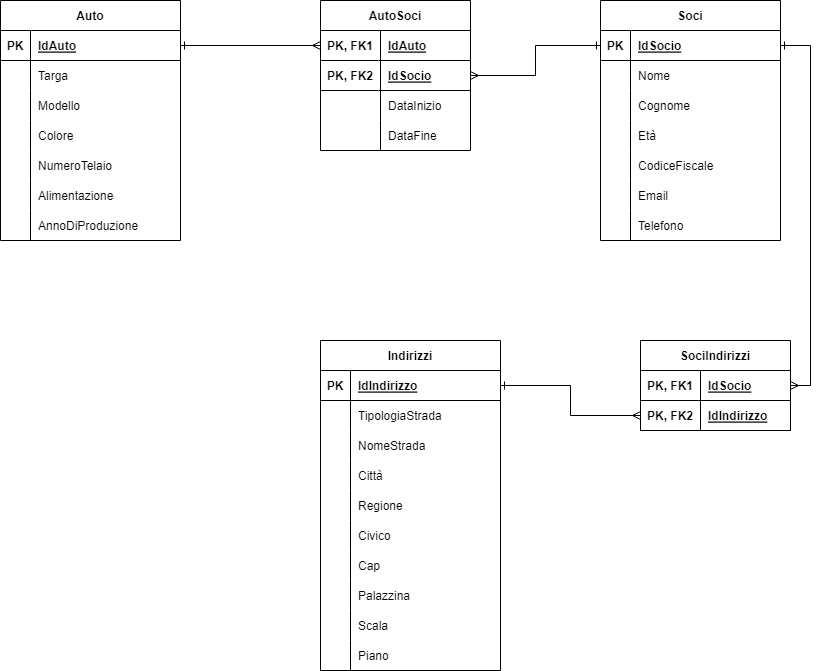
\includegraphics[width=16cm]{modello_logico_car_sharing.png}
    \label{fig:modello Logico}
    \caption{Rappresentazione modello Logico}
\end{figure}

\end{document}
